L'obiettivo del PT è trovare e utilizzare vulnerabilità all'interno
dell'applicativo web \textbf{OWASP Juice Shop}.

Oltre a questo report verranno allegati \textbf{i file di output dei
vari tool utilizzati}.

Metodologia

Di seguito descriviamo step-by-step le fasi del penetration test

\section{Information Gathering}\label{information-gathering}

\emph{Tecniche e strumenti utilizzati per raccogliere informazioni
iniziali.}

Abbiamo iniziato utilizzando \emph{Nmap} per fare \textbf{Service
Enumeration}, specificando l'ip della web app e la porta con il comando:

\emph{sudo nmap -p3000 -sV -O 172.17.0.2}

senza però ottenere risultati utili (file: \textbf{nmapOutput.txt}).

Per cercare di trovare qualche tecnologia utilizzata (con relative
versioni) abbiamo utilizzato Wappalyzer, ottenendo:

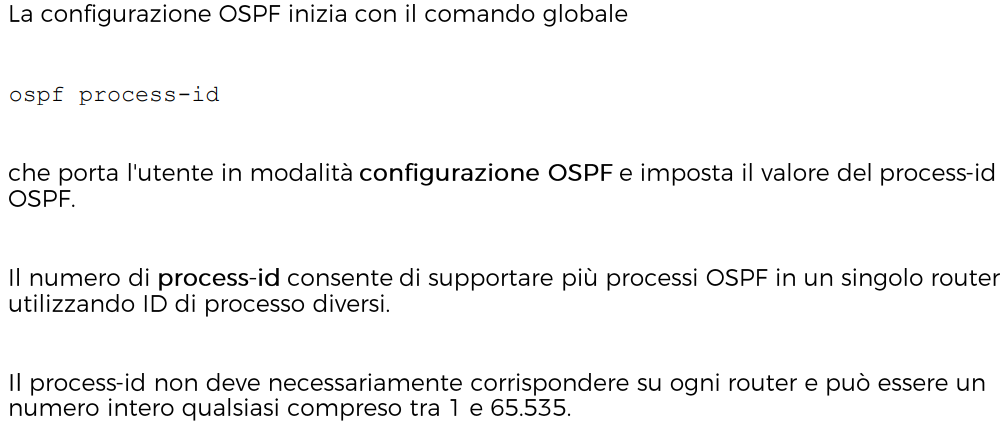
\includegraphics[width=3.7151in,height=3.46455in]{media/image4.png}

Dal tool otteniamo solo 3 versioni, e cercando nel web vulnerabilità
specifiche troviamo:

\begin{itemize}
\item
  \textbf{Angular 15.2.10}: nessuna vulnerabilità;
\item
  \hl{\textbf{jQuery 2.2.4}: vulnerabile ad attacchi di tipo
  \emph{Cross-site Scripting (XSS)};}
\item
  \textbf{core-js 3.37.1}: nessuna vulnerabilità.
\end{itemize}

In sostanza terremo utile questa unica informazione per le fasi
successive.

Un altro tool utilizzabile per scovare informazioni sulla web app è
\emph{WhatWeb}:

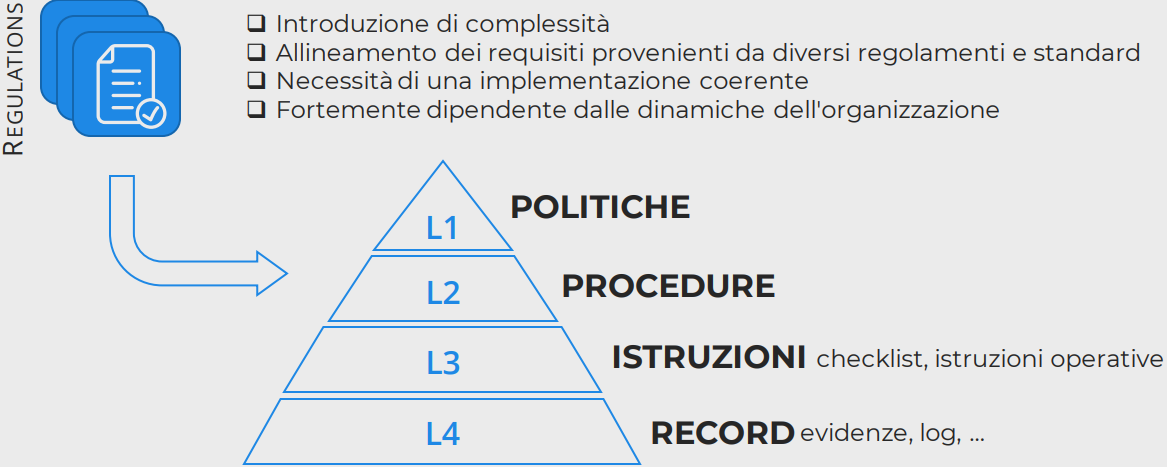
\includegraphics[width=6.27083in,height=0.31944in]{media/image18.png}

Il passo successivo è controllare, tramite \emph{WAFW00F}, se
l'applicazione ha un WAF (Web Application Firewall), e tramite il
comando:

\emph{wafw00f
\href{http://172.17.0.2:3000}{\ul{http://172.17.0.2:3000}}}

abbiamo ottenuto una risposta negativa che quindi ci conferma che non è
presente un WAF (file: \textbf{outputWafw00f.txt}).

Per avere un ulteriore conferma che le risposte http non vengano
alterate e capire se c'è uno strumento di detection/response tramite
l\textquotesingle utilizzo di Wireshark abbiamo filtrato le risposte
HTTP, notando che la prima richiesta fatta è classica, per poi andare ad
eseguire altre richieste con dei failed, ad esempio ``Ealert''.

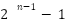
\includegraphics[width=6.08395in,height=1.41667in]{media/image10.png}

Per cercare alcuni path o file interessanti abbiamo usato \emph{Nikto},
ottenendo un gran numero di falsi positivi ma anche risultati (file:
\textbf{outputNikto}), in particolare:

\begin{itemize}
\item
  \emph{/ftp}: contiene molti file non leggibili, ma tra quelli
  leggibili abbiamo ``\textbf{acquisitions.md}'' un file confidenziale.
  L'apertura dei file non leggibili ci permette di scoprire, tramite
  errore, che la web app usa \textbf{\hl{Express 4.17.1}};
\end{itemize}

\begin{quote}
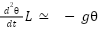
\includegraphics[width=5.46354in,height=1.3432in]{media/image31.png}
\end{quote}

\emph{\hl{Vulnerabile ad attacchi di tipo \textbf{Open Redirect}}}

\begin{itemize}
\item
  \emph{/ftp/quarantine}: directory con malware per diversi OS;
\end{itemize}

\begin{quote}
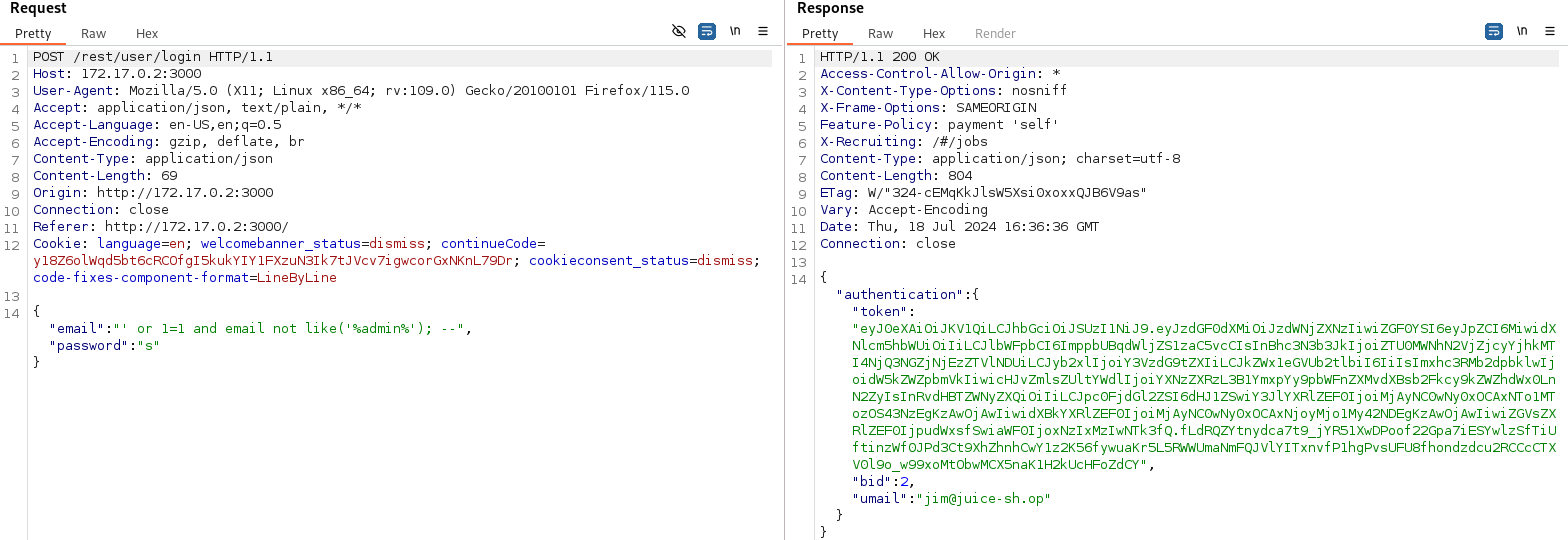
\includegraphics[width=6.26772in,height=0.61111in]{media/image29.png}
\end{quote}

Successivamente siamo passati alla pagina di login cercando, in qualche
modo, di provocare errori che ci avrebbero dato indizi sulle tecnologie
o metodologie utilizzate nel backend.

Inserendo caratteri inaspettati dalla form, come per esempio il singolo
apice, abbiamo ottenuto un errore diverso dal solito, che ci fa capire
come probabilmente c'è un problema che potrebbe portarci ad una
vulnerabilità.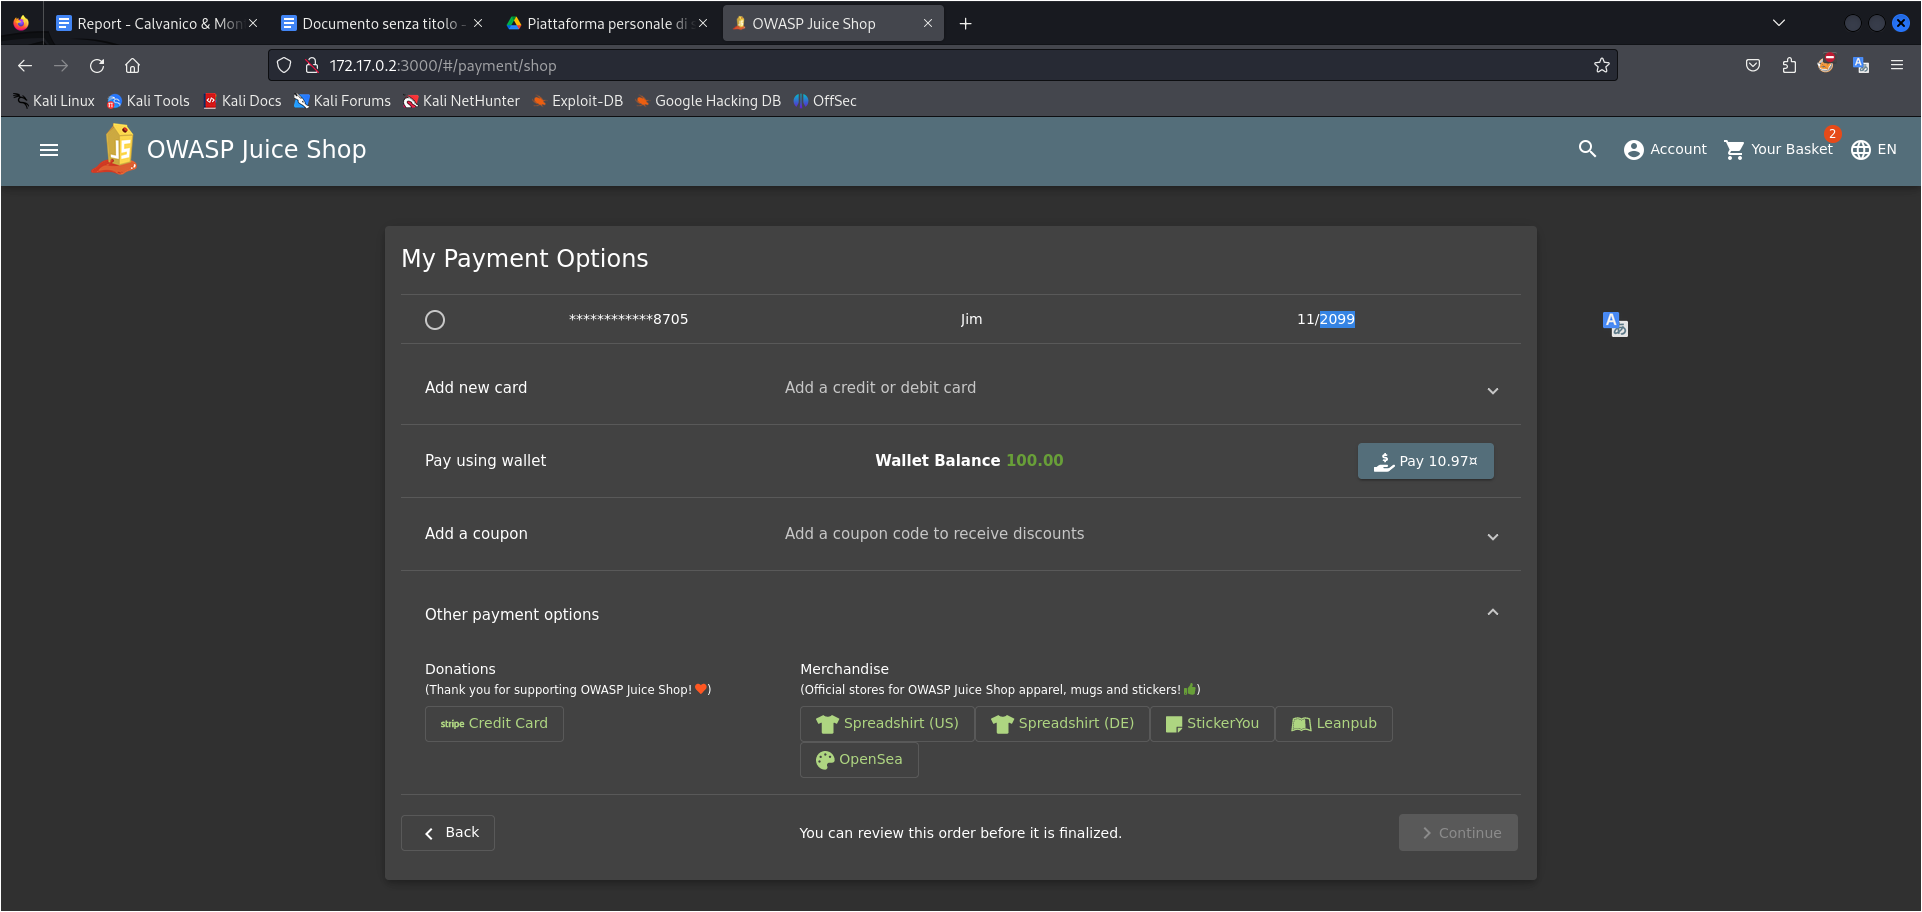
\includegraphics[width=6.26772in,height=2.33333in]{media/image12.png}

Nella parte di vulnerability assessment indagheremo meglio.

Il passo successivo è stato quello di trovare nuove directory e
sottodirectory tramite tool automatizzati, nel nostro caso \emph{Ffuf}
(file: \textbf{outputFfuf}), dove tramite comando:

\emph{ffuf -u http://172.17.0.2:3000/FUZZ -w
/usr/share/dirbuster/wordlists/directory-list-1.0.txt -fs 3740-3750}

abbiamo cercato all'interno della web app tutti i possibili percorsi,
passandogli una wordlist (contenuta nativamente dentro kali) con parole
chiave da cercare e togliendo tutti i risultati che ritornavano una size
compresa tra quella inserita (la size della homepage); questo perché il
sito ritorna la pagina iniziale ogni volta che si prova ad accedere ad
un indirizzo inesistente.

Tra i path trovati quelli effettivamente raggiungibili e interessanti
sono:

\begin{itemize}
\item
  \emph{/restoration}: path che ritorna un errore e come i precedenti ci
  da informazioni sul backend;
\item
  \emph{/apictureofbritain}: come il precedente
\item
  \emph{/video}: ci mostra un video altrimenti non raggiungibile;
\item
  \hl{\emph{/metrics}: un'insieme di metriche di nodejs};
\item
  \hl{\emph{/redirect}: da questo path se aggiunto \emph{?to=} è
  possibile arrivare a parti altrimenti non raggiungibili, questo perchè
  i bottoni utilizzano questa combinazione per portare in altre pagine,
  tramite Burp lo possiamo
  dimostrare}.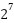
\includegraphics[width=4.35417in,height=1.40625in]{media/image11.png}
\end{itemize}

Notando che alcune pagine contenevano nel path: \emph{/\#/nome} abbiamo
pensato di fare nuove scansioni (file: \textbf{outputFfuf2.txt)}, sempre
con fuff però usando un link diverso e con delle wordlist differenti
(relative al tool):

\emph{ffuf -u http://172.17.0.2:3000/\#/FUZZ -w
/usr/share/wfuzz/wordlists/common.txt -o outputFfuf2.txt}

In questo caso abbiamo tolto il filtro perché con esso non dava
risultati.

Togliendo il filtro otteniamo molti falsi positivi, ma dopo aver
controllato alcuni path interessanti abbiamo trovato:

\begin{itemize}
\item
  \hl{\emph{/administration}: il path ritorna errore 403, questo vuol
  dire che esiste ma non è accessibile senza permessi, sarà da
  ricontrollare dopo aver fatto l'accesso};
\end{itemize}

Infine controlliamo anche i cookie per cercare nei flag eventuali
parametri non conformi da utilizzare per scovare vulnerabilità, senza
però riscontrare nulla di anomalo.

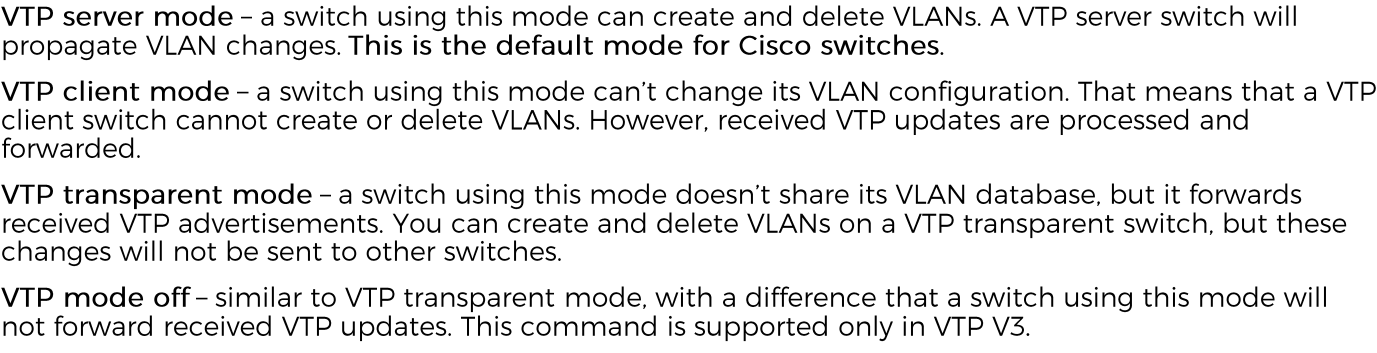
\includegraphics[width=5.59722in,height=3.51198in]{media/image22.png}

\section{Vulnerability Assessment}\label{vulnerability-assessment}

\emph{Strumenti e metodi per identificare le vulnerabilità.}

Abbiamo iniziato la fase indagando l'errore anomalo ottenuto dalla form,
usando il \emph{Repeater di Burp}, per modificare le richieste di log in
maniera più veloce e per ottenere le risposte complete, abbiamo inserito
dei caratteri inaspettati generando questo errore:

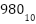
\includegraphics[width=5.22712in,height=5.04688in]{media/image32.png}

andando a scoprire \hl{esattamente la query utilizzata e che viene
utilizzato SQLite}.

In questo modo potremmo fare un attacco di tipo \textbf{sql injection}
per poter accedere con un account.

\section{Exploitation}\label{exploitation}

\emph{Tentativi di sfruttamento delle vulnerabilità trovate.}

Dopo aver riscontrato nella fase precedente che la vulnerabilità nel
login esiste abbiamo eseguito un attacco di tipo \emph{SQL Injection,}
andando ad inserire nel campo email:

\emph{admin' or 1=1 --}

permettendoci di accedere con l\textquotesingle account admin, questo
perché l'email verrà sempre considerata vera (grazie al 1=1) e la
password verrà saltata, andando a prendere il primo account salvato del
DB.

Con questa informazione, e una conoscenza pregressa di SQL, abbiamo
provato a trovare altri account con cui accedere utilizzando un altro
mezzo messo a disposizione da SQL stesso: il \textbf{LIKE}.

Nel dettaglio abbiamo impostato un attacco \emph{SQL Injection}
inserendo nella form:

\emph{admin' or 1=1 and email not like(`\%admin\%'); --}

\emph{{[}I \% contano come segnaposto all'interno di SQL{]}}

in questo modo otterremo accesso all'account successivo, che in questo
caso è Jim:

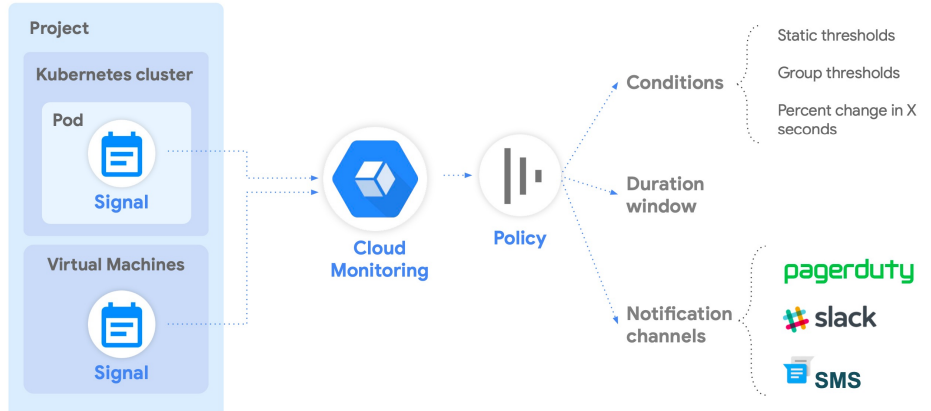
\includegraphics[width=6.26772in,height=2.15278in]{media/image28.png}

Continuando su questa strada abbiamo fatto:

\emph{admin' or 1=1 and email not like(`\%admin\%') and email not
like(`\%jim\%'); --}

ottenendo accesso ad un altro account denominato Bender:

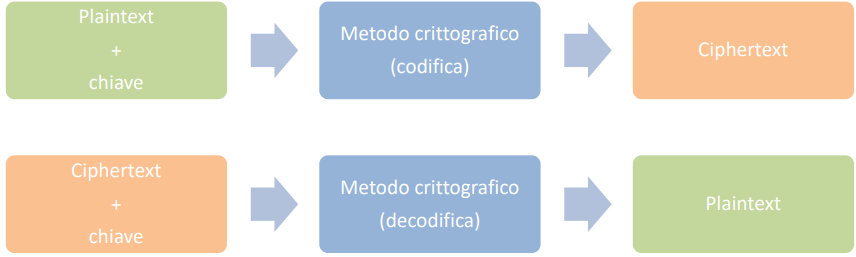
\includegraphics[width=6.26772in,height=2.16667in]{media/image19.png}

Andando avanti così è possibile accedere a tutti gli account esistenti,
creando non pochi problemi.

Ricordandoci dalla fase di information gathering che il sito usa jQuery
versione 2.2.4 sappiamo che è vulnerabile ad attacchi di tipo Cross-site
Scripting (XSS).

Tramite questa informazione possiamo provare ad inserire codice
javascript e tag html in tutte quelle parti che accettano input
dall'utente.

Se per esempio nella barra di ricerca mettiamo tag html e/o codice
javascript questo viene inserito senza nessun tipo di controllo,
ottenendo questi risultati:

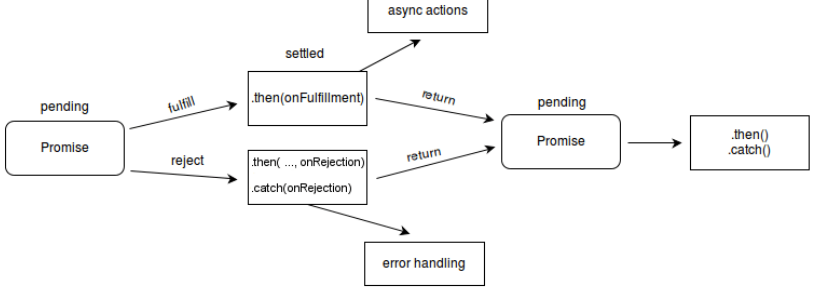
\includegraphics[width=6.26772in,height=0.70833in]{media/image7.png}

Questo inserendo \emph{\textless button\textgreater Click
Me!\textless/button\textgreater{}}.

Oppure inserendo \emph{\textless iframe src="javascript:alert(`Molto
male\ldots`)"\textgreater{}}:

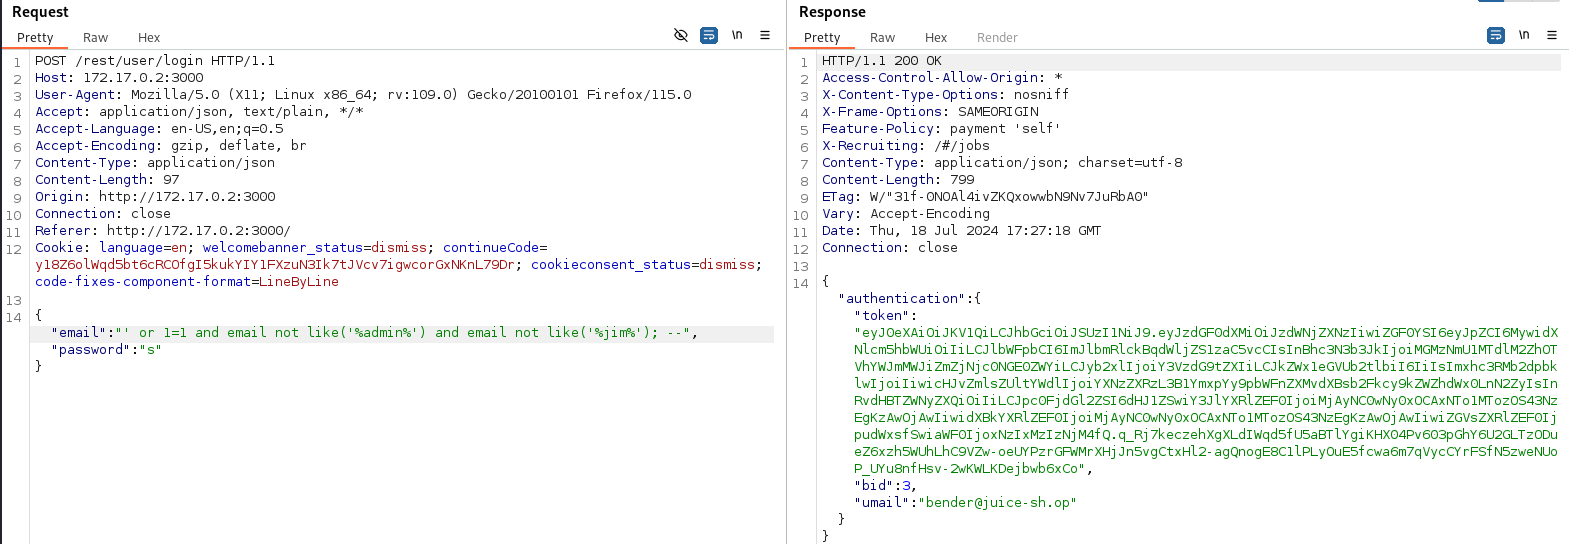
\includegraphics[width=6.26772in,height=2.41667in]{media/image16.png}

\section{Post-Exploitation}\label{post-exploitation}

\emph{Azioni compiute dopo l\textquotesingle accesso iniziale.}

Dopo aver ottenuto l'accesso all'account admin siamo andati a
controllare il path trovato nella fase di \textbf{Information
Gathering}, \emph{\hl{/administration}}, che era inaccessibile senza
permessi.

In questa sezione possiamo vedere tutti gli account e anche tutte le
recensioni rilasciate, con la possibilità di rimuoverle.

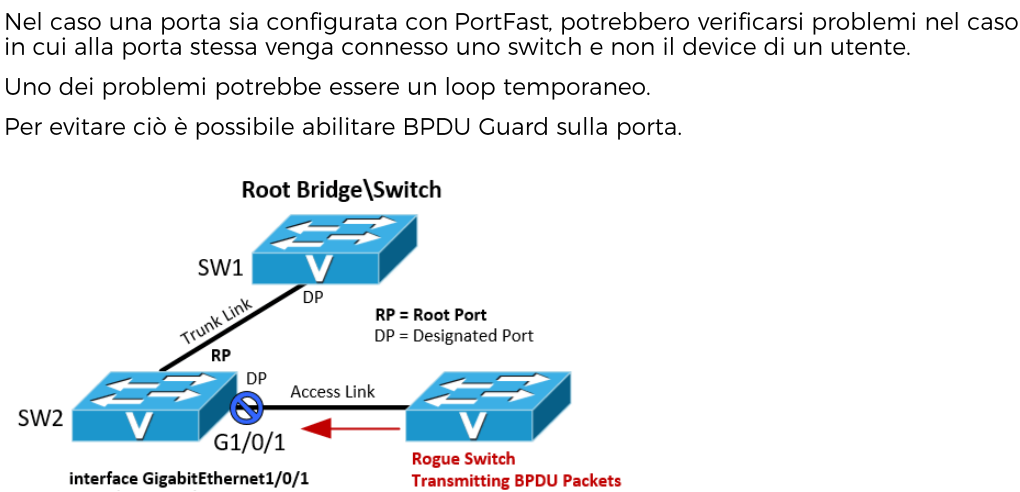
\includegraphics[width=3.54843in,height=3.97786in]{media/image15.png}

Successivamente abbiamo iniziato a controllare le varie pagine
disponibili solo ad un account registrato.

La nostra attenzione è passata subito alla sezione ``\emph{Your
Basket}'', che nell'account admin conteneva già dei prodotti:

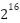
\includegraphics[width=4.92188in,height=3.0169in]{media/image3.png}

Andando a controllare come questi dati vengono salvati anche alla
chiusura della pagina o al cambio di schermata abbiamo aperto la sezione
Storage nello strumento degli sviluppatori del browser; questo grazie
alle conoscenze pregresse ottenute durante un altro corso, dove abbiamo
creato anche noi una web app per ordinare prodotti.

Nello specifico abbiamo controllato il \emph{Local e Session Storage:}

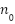
\includegraphics[width=6.26772in,height=0.98611in]{media/image17.png}

Il Local contiene il token di autenticazione.

Invece il Session i dettagli del carrello:

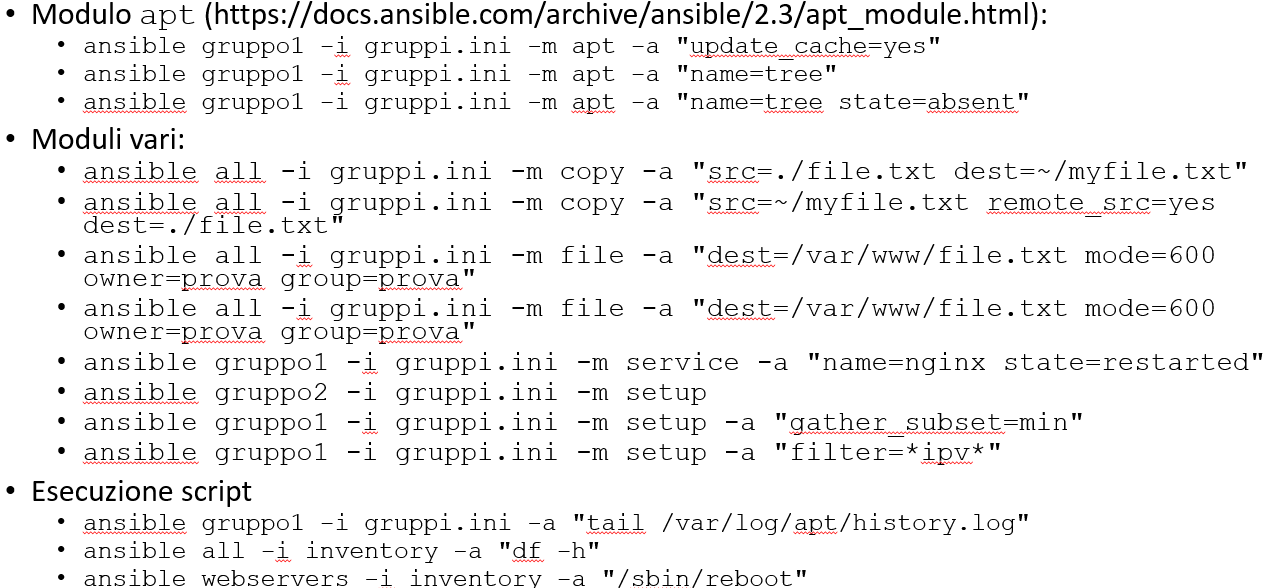
\includegraphics[width=6.26772in,height=0.98611in]{media/image2.png}

I due valori che ci sono subito caduti sott\textquotesingle occhio sono
il prezzo totale (\emph{itemTotal}) e l'id del carrello (\emph{bid}).

Andando a modificare il primo a 0 per provare a non pagare i prodotti
notiamo, come giusto che sia, che il valore viene ricalcolato rendendo
impossibile questo trucco.

Modificando invece il \emph{bid} possiamo accedere ad altri carrelli:

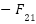
\includegraphics[width=5.27239in,height=2.68413in]{media/image14.png}

Riuscendo anche a fare il checkout:

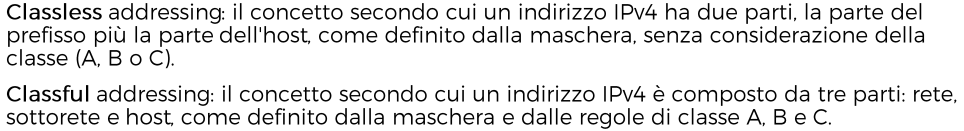
\includegraphics[width=5.40383in,height=2.83213in]{media/image6.png}

Sapendo dalla fase di Information Gathering che la web app utilizza il
``redirect?to'' per reindirizzare verso altre pagine, abbiamo deciso di
fare una ricerca all'interno del file \emph{main.js} per trovare tutti
gli utilizzi.

Utilizzando il dev tool del browser abbiamo cercato tramite Ctrl+F tutte
le occorrenze del redirect nel file di script, trovando un redirect che
normalmente non sarebbe accessibile.

L'URL ritorna a un crypto wallet che probabilmente veniva utilizzato per
ricevere donazioni.
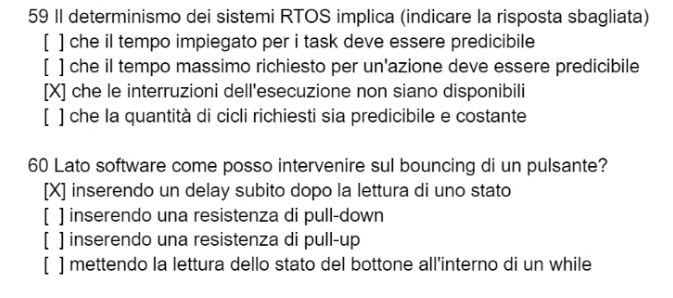
\includegraphics[width=6.26772in,height=1.15278in]{media/image21.png}

Andando a ritroso cercando dove venga utilizzata la funzione
\emph{showBitcoinQrCode} possiamo notare che viene chiamata nella parte
di gestione del carrello, ma nella web app non è presente.

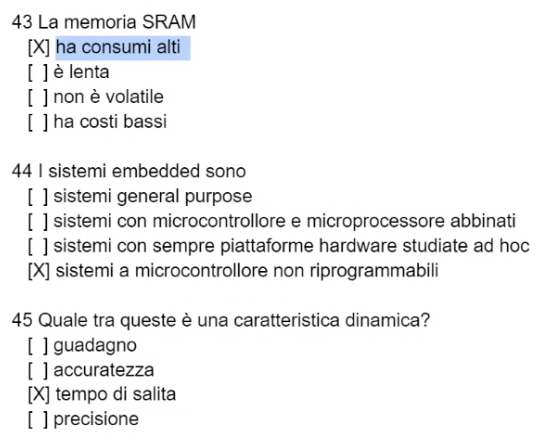
\includegraphics[width=3.84743in,height=2.19792in]{media/image8.png}

Strumenti Utilizzati

\section{Burp Suite}\label{burp-suite}

\subsection{Motivo
dell\textquotesingle utilizzo}\label{motivo-dellutilizzo}

Lo strumento ci aiuta con un Proxy per intercettare e successivamente
visualizzare le richieste della web app.

A differenza degli strumenti degli sviluppatori integrati nel browser,
Burp è più flessibile, permettendo di modificare le richieste,
visualizzarle nella sezione Logger, ecc.

\subsection{Obiettivo della scansione}\label{obiettivo-della-scansione}

L'obiettivo è cercare nelle richieste informazioni utili per individuare
vulnerabilità ed effettuare exploit.

\subsection{Spiegazione del
funzionamento}\label{spiegazione-del-funzionamento}

Burp intercetta e blocca le richieste verso e da la web app, questo è
possibile perché abbiamo installato un\textquotesingle estensione nel
browser utilizzato (FireFox), chiamata FoxyProxy, che implementa un
proxy che ri-indirizza le richieste verso Burp permettendoci di
interagire con esse.

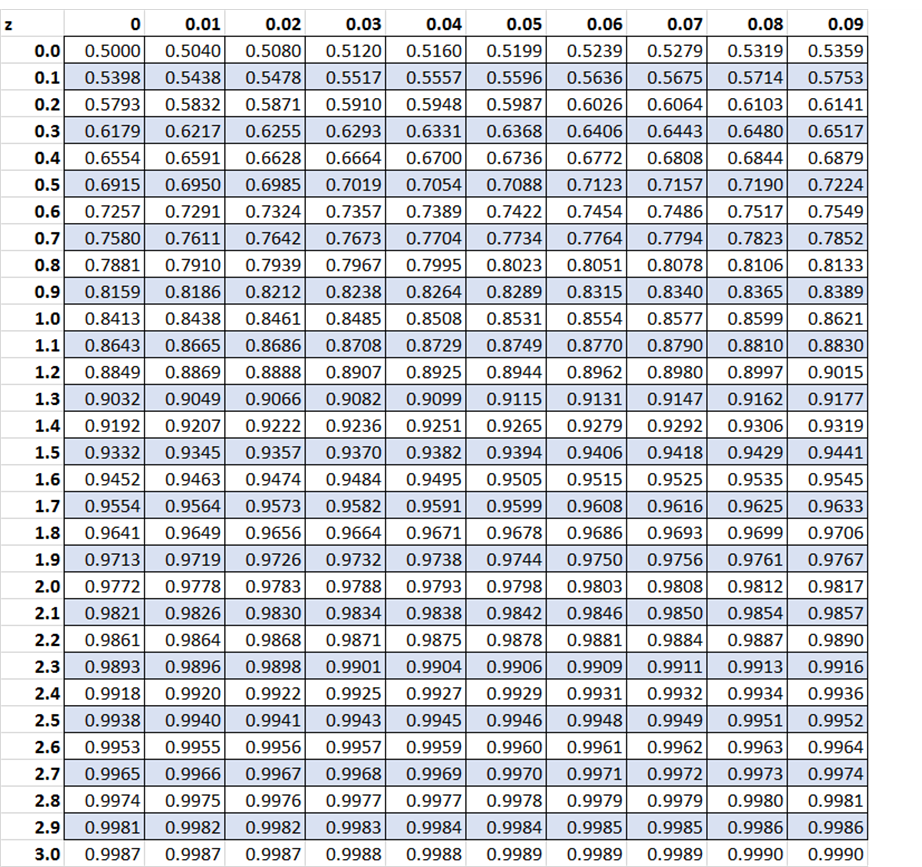
\includegraphics[width=6.26772in,height=5.15278in]{media/image9.png}

\section{Nmap}\label{nmap}

\subsection{Motivo
dell\textquotesingle utilizzo}\label{motivo-dellutilizzo-1}

Utilizzato per fare service enumeration, specifichiamo l'ip + porta e il
tool ci restituisce i servizi, con rispettive versioni utilizzate.

\subsection{Obiettivo della
scansione}\label{obiettivo-della-scansione-1}

Scoprire che servizi vengono utilizzati dalla web app con anche la
versione per cercare possibili vulnerabilità.

\subsection{Spiegazione del
funzionamento}\label{spiegazione-del-funzionamento-1}

Tramite comando:

\emph{nmap -p{[}PORT{]} {[}FLAG{]} {[}IP{]}}

il tool invia pacchetti al host e in base alla risposta capisce se una
porta è aperta, filtrata o chiusa e quindi se un servizio è utilizzato o
meno oppure può ottenere informazioni sul OS.

\section{Wappalyzer}\label{wappalyzer}

\subsection{Motivo
dell\textquotesingle utilizzo}\label{motivo-dellutilizzo-2}

Utilizzato per ottenere informazioni sulle tecnologie utilizzate dal
sito e relative versioni

\subsection{Obiettivo della
scansione}\label{obiettivo-della-scansione-2}

Trovare tecnologie vulnerabili nella web app in modo da fare l'exploit
su di esse.

\subsection{Spiegazione del
funzionamento}\label{spiegazione-del-funzionamento-2}

il tool cerca negli header http, nel codice html e script informazioni
che potrebbero ritornare a certe tecnologie e versioni.

\section{WAF00F}\label{waf00f}

\subsection{Motivo
dell\textquotesingle utilizzo}\label{motivo-dellutilizzo-3}

Tool perfetto per controllare la presenza di WAF in maniera veloce e
senza troppe configurazioni.

\subsection{Obiettivo della
scansione}\label{obiettivo-della-scansione-3}

Trovare che tipo di WAF viene usato in modo da sapere quale tipo di
traffico viene bloccato o meno, utile per usare certi exploit.

\subsection{Spiegazione del
funzionamento}\label{spiegazione-del-funzionamento-3}

Tramite comando:

\emph{waf00f {[}INDIRIZZO{]}}

invia una serie di richieste HTTP a un sito web e analizza le risposte
per identificare il WAF in uso.

\section{Wireshark}\label{wireshark}

\subsection{Motivo
dell\textquotesingle utilizzo}\label{motivo-dellutilizzo-4}

Fare lo sniff dei pacchetti HTTP verso e dalla web app.

\subsection{Obiettivo della
scansione}\label{obiettivo-della-scansione-4}

Prova manuale per avere un\textquotesingle ulteriore conferma che le
risposte HTTP non vengano alterate da uno strumento di
detection/response.

\subsection{Spiegazione del
funzionamento}\label{spiegazione-del-funzionamento-4}

Il tool intercetta i pacchetti in arrivo e verso un obiettivo con la
possibilità di filtrarli.

\section{Nikto}\label{nikto}

\subsection{Motivo
dell\textquotesingle utilizzo}\label{motivo-dellutilizzo-5}

Come automatic scanners è veloce e applicabile a qualsiasi realtà.

\subsection{Obiettivo della
scansione}\label{obiettivo-della-scansione-5}

Trovare path che non dovrebbero essere accessibili dagli utenti in modo
da scovare informazioni sensibili.

\subsection{Spiegazione del
funzionamento}\label{spiegazione-del-funzionamento-5}

Tramite comando:

\emph{nikto -host{[}INDIRIZZO{]}}

il tool ricerca informazioni sul web server o
sull\textquotesingle applicazione web da scansionare; successivamente
inizia la scansione utilizzando richieste http e file.

\section{FFUF}\label{ffuf}

\subsection{Motivo
dell\textquotesingle utilizzo}\label{motivo-dellutilizzo-6}

Abbiamo scelto questo tool invece che altri, con lo stesso scopo, perché
più veloce e con tanti flag utili per personalizzare la ricerca.

\subsection{Obiettivo della
scansione}\label{obiettivo-della-scansione-6}

Trovare nuove sottodirectory per scovare vulnerabilità o tecnologie
usate dalla web app.

\subsection{Spiegazione del
funzionamento}\label{spiegazione-del-funzionamento-6}

Tramite comando:

\emph{ffuf -u{[}INDIRIZZO{]} -w{[}PATH WORDLIST{]} -fs{[}SIZE
RISPOSTA{]}}

il tool parte dal rootdir e ricerca ricorsivamente su ogni
sottodirectory trovata; i due flag utilizzati fanno:

\begin{itemize}
\item
  \textbf{-w}: prende una wordlist dal path inserito;
\item
  \textbf{-fs}: filtra le risposte in base al size del ritorno, ci è
  servito perché la webapp in caso di indirizzo errato ritorna la pagina
  iniziale.
\end{itemize}

Analisi delle Vulnerabilità

\section{SQL Injection - Login}\label{sql-injection---login}

\subsection{Descrizione della
vulnerabilità}\label{descrizione-della-vulnerabilituxe0}

Tramite l'inserimento di certi caratteri e stringhe tipiche di SQL, e
inaspettati dal server, è possibile eseguire codice malevolo.

In questo caso usata per ottenere accesso ad uno o più account (tra cui
quello dell'admin).

\subsection{Riproducibilità}\label{riproducibilituxe0}

Per riprodurre la vulnerabilità bisogna:

\begin{enumerate}
\def\labelenumi{\arabic{enumi}.}
\item
  andare nella pagine di login;
\item
  inserire la seguente stringa nell'email: \emph{Placeholder' or 1=1
  --};
\item
  inserire qualunque cosa nella password;
\item
  cliccare invio.
\end{enumerate}

In sostanza va messo dopo l'or una condizione sempre vera, seguito dai
simboli per commentare.

\subsection{Prova della rilevazione}\label{prova-della-rilevazione}

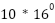
\includegraphics[width=6.26772in,height=1.98611in]{media/image24.png}

\subsection{Classificazione OWASP TOP
10}\label{classificazione-owasp-top-10}

Secondo l'OWASP questo tipo di vulnerabilità è classificata:

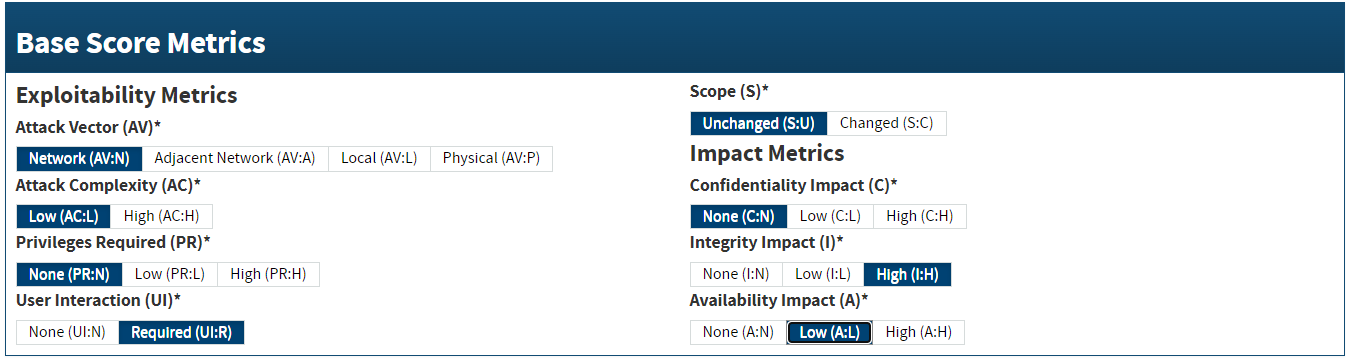
\includegraphics[width=6.26772in,height=2.83333in]{media/image26.png}

Lo score del CVSS è:

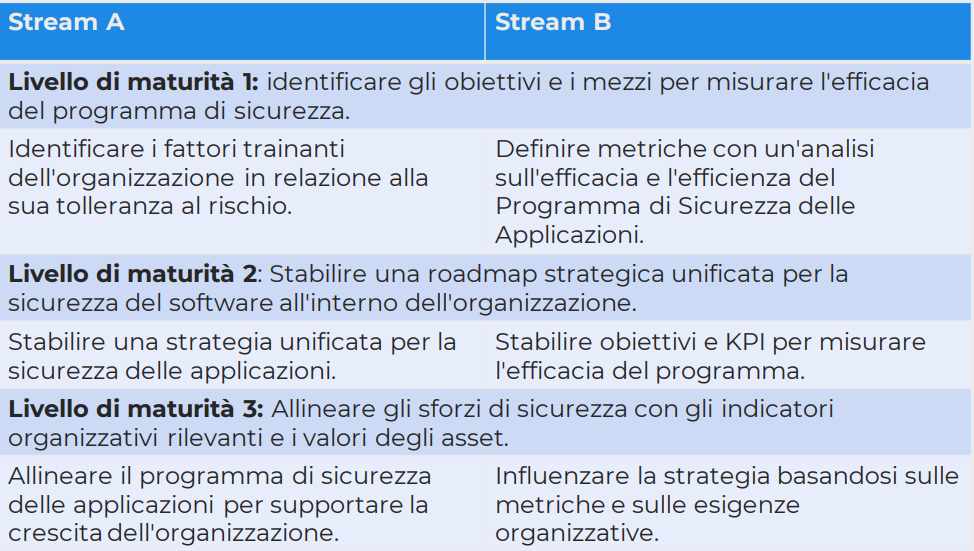
\includegraphics[width=3.8765in,height=1.93825in]{media/image13.png}

Con le seguente metriche:

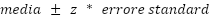
\includegraphics[width=6.26772in,height=1.65278in]{media/image1.png}

\subsection{Requisiti
dell\textquotesingle attaccante}\label{requisiti-dellattaccante}

L'unica cosa necessaria è avere accesso al sito web e una conoscenza di
SQL.

\subsection{Gravità e Impatti}\label{gravituxe0-e-impatti}

Questa vulnerabilità è estremamente grave, perché permette di accedere
come admin all'applicativo web con un impatto non indifferente
sull'integrità dell'applicativo e dei dati.

\section{XSS - DOM}\label{xss---dom}

\subsection{Descrizione della
vulnerabilità}\label{descrizione-della-vulnerabilituxe0-1}

Un Cross-Site Scripting è una vulnerabilità che permette a un
malintenzionato di iniettare codice dannoso all\textquotesingle interno
di un sito web legittimo.

\subsection{Riproducibilità}\label{riproducibilituxe0-1}

Nel nostro caso tramite il campo ricerca siamo riusciti ad inserire nel
DOM componenti HTML, come bottoni e alert, ecco gli step:

\begin{enumerate}
\def\labelenumi{\arabic{enumi}.}
\item
  aprire il campo ricerca;
\item
  inserire qualunque tag si voglia, nel nostro caso:
  \emph{\textless iframe src="javascript:alert(`Molto
  male\ldots`)"\textgreater{}};
\item
  all'invio si vedrà nel DOM della pagina il tag inserito nel campo di
  input.
\end{enumerate}

\subsection{Prova della rilevazione}\label{prova-della-rilevazione-1}

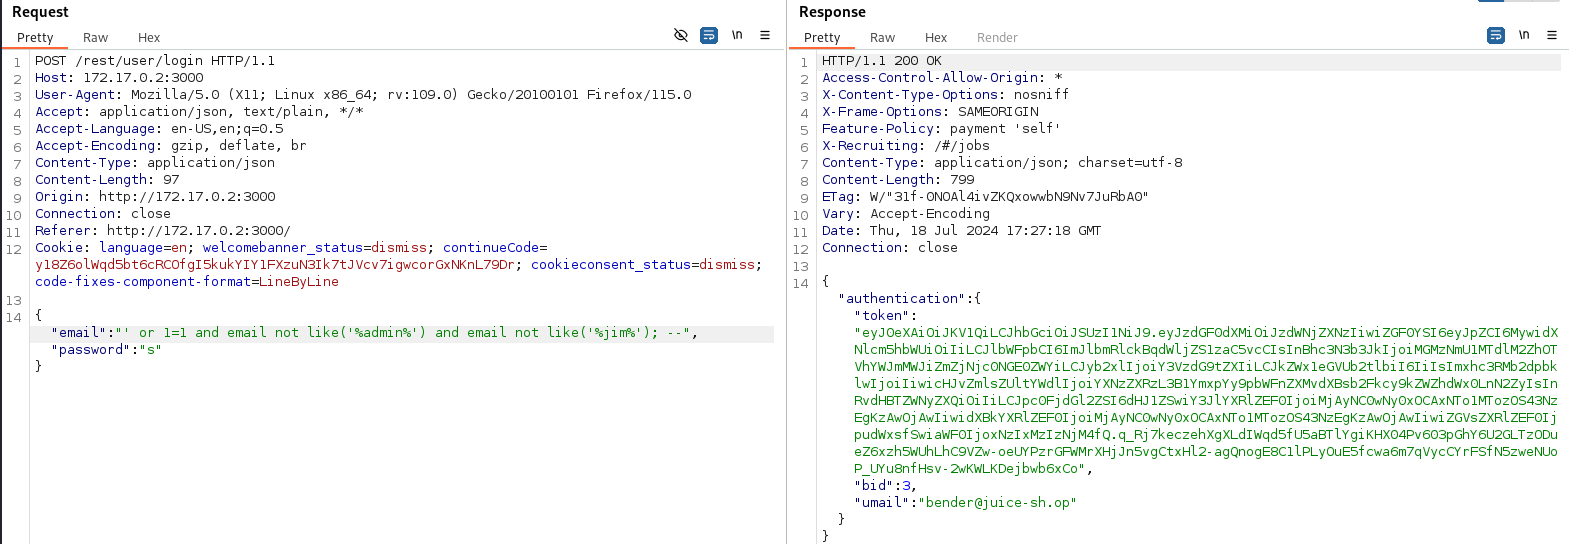
\includegraphics[width=6.26772in,height=2.41667in]{media/image16.png}

\subsection{Classificazione OWASP TOP
10}\label{classificazione-owasp-top-10-1}

Secondo l'OWASP questo tipo di vulnerabilità è classificata:

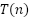
\includegraphics[width=6.26772in,height=2.05556in]{media/image5.png}

Lo score del CVSS è:

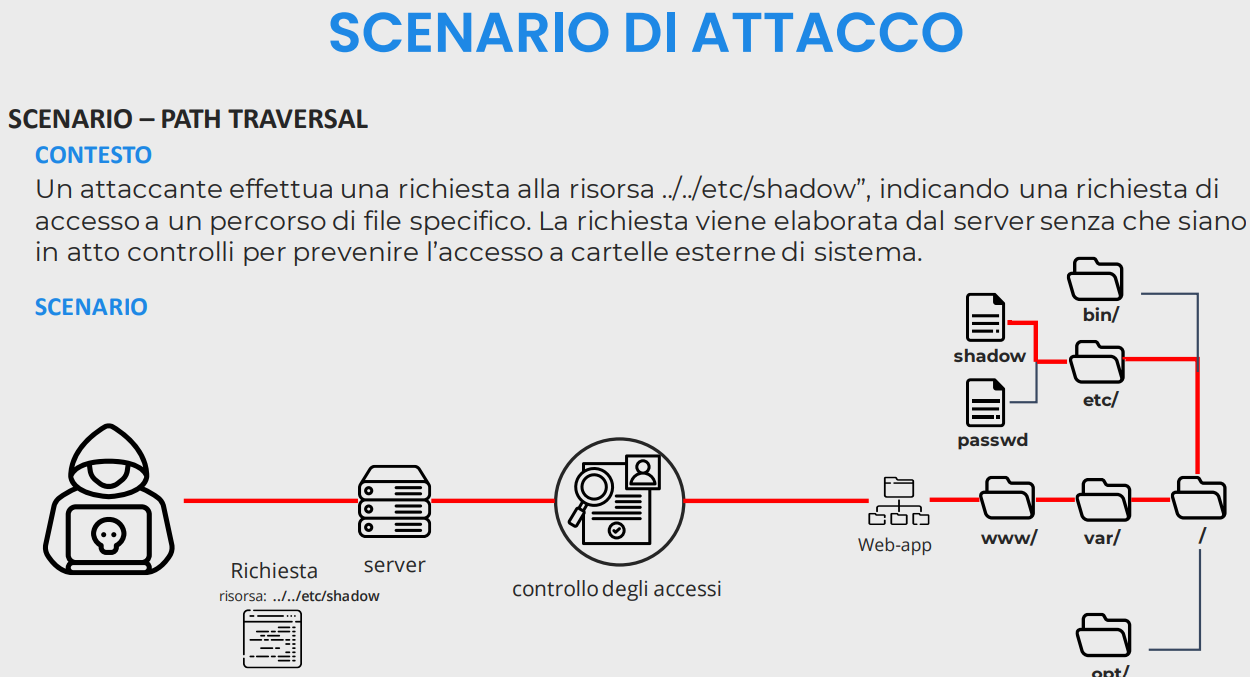
\includegraphics[width=2.96573in,height=1.42153in]{media/image30.png}

Con le seguente metriche:

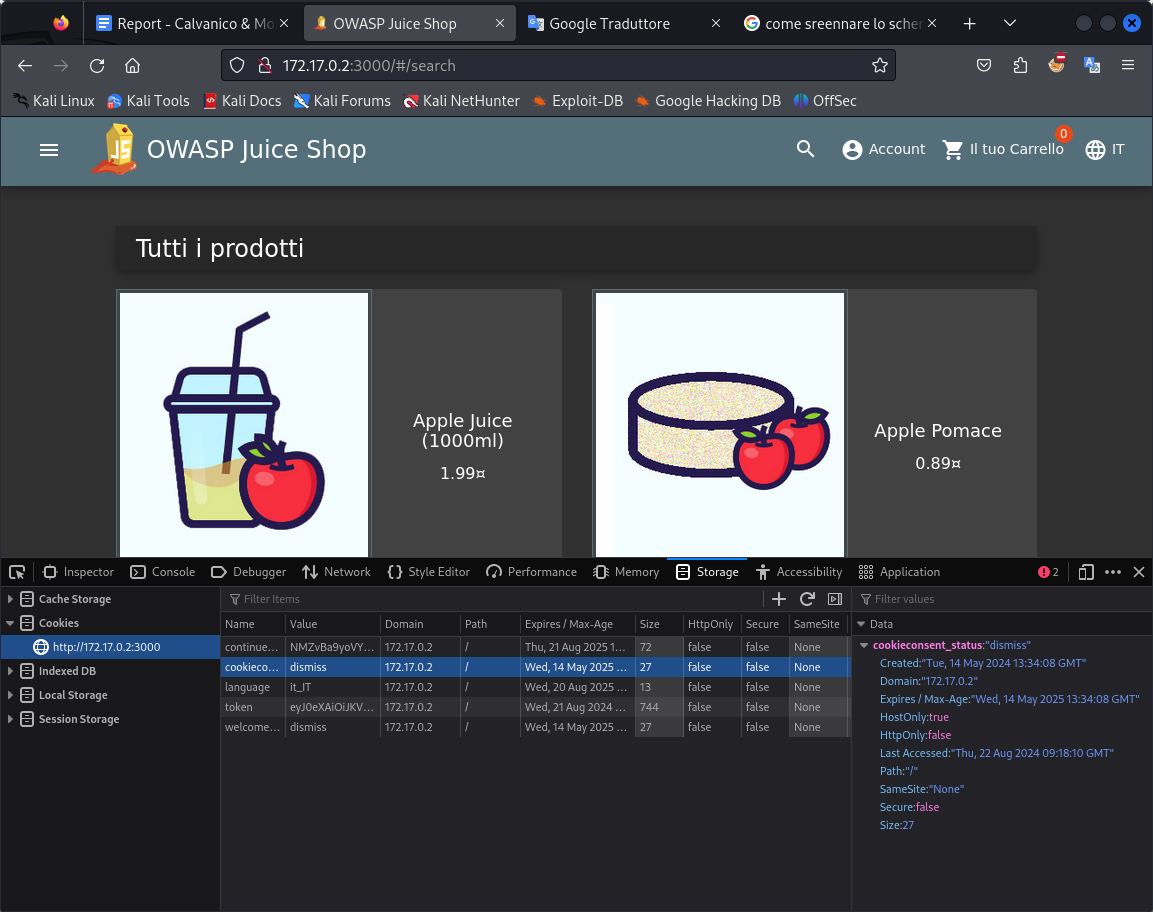
\includegraphics[width=6.26772in,height=1.66667in]{media/image25.png}

\subsection{Requisiti
dell\textquotesingle attaccante}\label{requisiti-dellattaccante-1}

L'attaccante deve solo aver accesso alla web app e conoscere un minimo
di html.

\subsection{Gravità e Impatti}\label{gravituxe0-e-impatti-1}

Se la modifica, che viene fatta tramite questa vulnerabilità, rimane
salvata all'interno della pagina il codice javascript verrà eseguito sul
browser dell'utente ad ogni accesso, creando situazioni altamente
pericolose.

La vulnerabilità ha una gravità moderata se il codice non viene salvato
(\emph{Reflected XSS}) con impatti medio/bassi, al contrario si ha una
gravità e un impatto critici.

\section{Broken Access Control - Accesso ad un altro
carrello}\label{broken-access-control---accesso-ad-un-altro-carrello}

\subsection{Descrizione della
vulnerabilità}\label{descrizione-della-vulnerabilituxe0-2}

Tramite una configurazione errata del Session Storage e dei permessi è
possibile accedere al carrello di un altro utente, con la possibilità di
effettuare tutte le normali attività.

\subsection{Riproducibilità}\label{riproducibilituxe0-2}

Per effettuare questa vulnerabilità è necessario:

\begin{enumerate}
\def\labelenumi{\arabic{enumi}.}
\item
  essere autenticati ad un account;
\item
  aprire il carrello e il dev tool del browser;
\item
  nella sezione \emph{Session Storage} cambiare il campo \emph{bid}
\end{enumerate}

\subsection{Prova della rilevazione}\label{prova-della-rilevazione-2}

Bid prima del cambio:

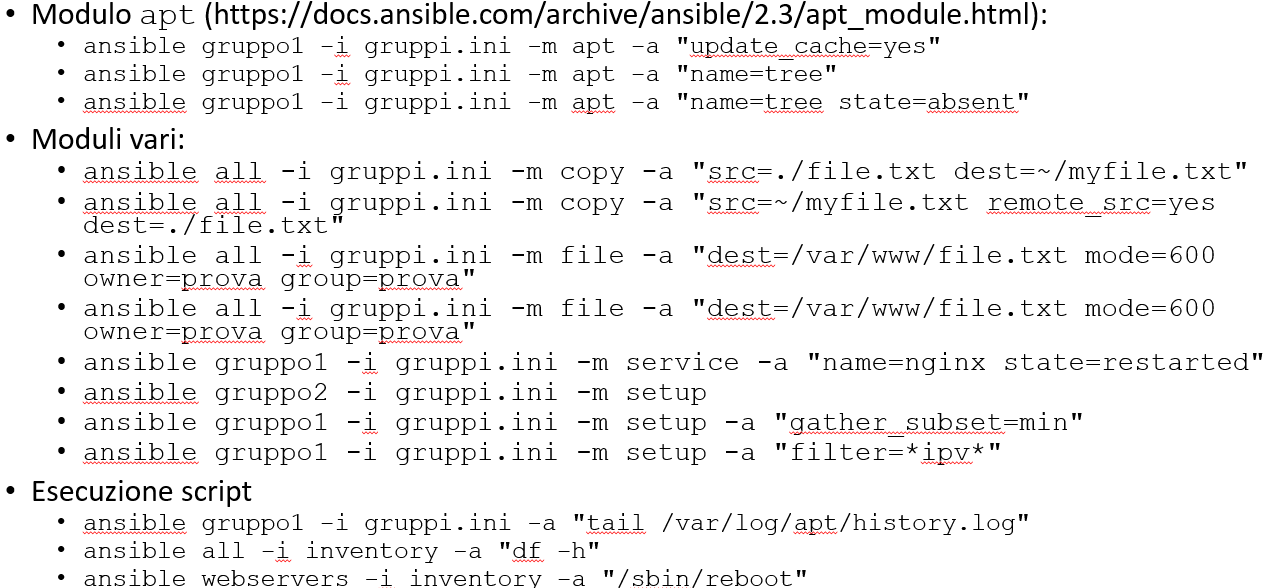
\includegraphics[width=6.26772in,height=0.98611in]{media/image2.png}

Bid e carrello dopo il cambio:

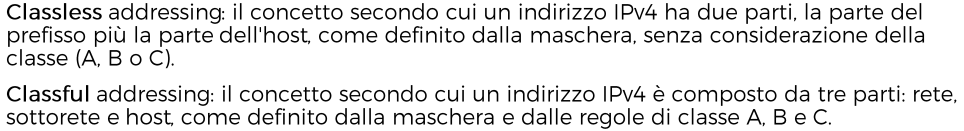
\includegraphics[width=6.26772in,height=3.23611in]{media/image6.png}

\subsection{Classificazione OWASP TOP
10}\label{classificazione-owasp-top-10-2}

Secondo l'OWASP questo tipo di vulnerabilità è classificata:

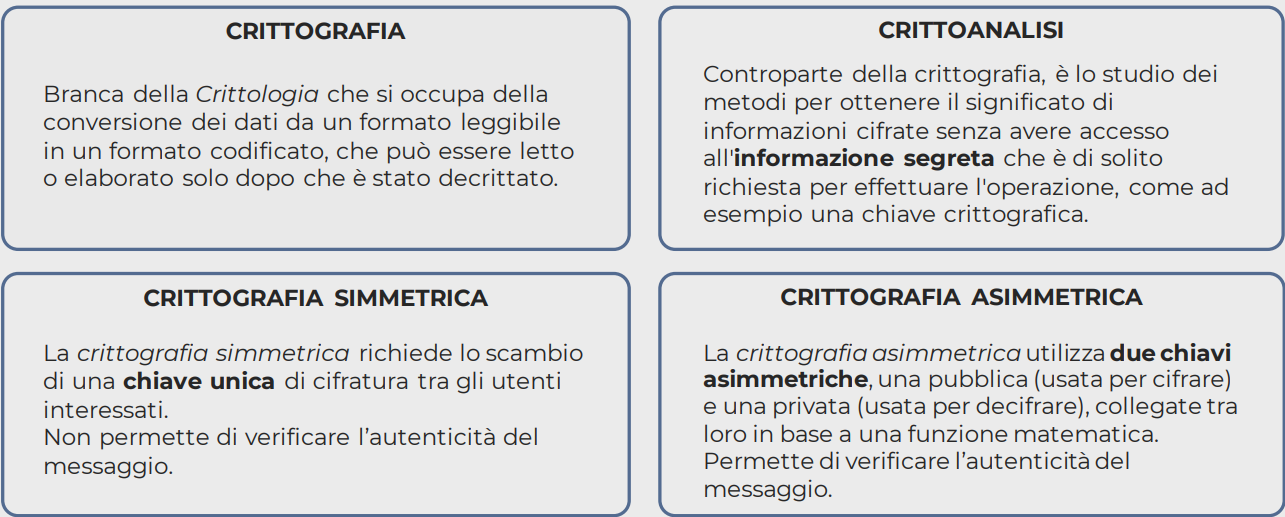
\includegraphics[width=6.26772in,height=2.61111in]{media/image20.png}

Lo score del CVSS è:

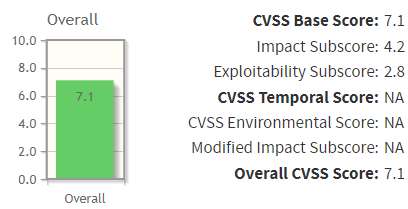
\includegraphics[width=4.25in,height=2.17708in]{media/image27.png}

Con le seguente metriche:

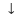
\includegraphics[width=6.26772in,height=1.65278in]{media/image23.png}

\subsection{Requisiti
dell\textquotesingle attaccante}\label{requisiti-dellattaccante-2}

L'attaccante deve avere un account con cui accedere al proprio carrello
e saper utilizzare il dev tool.

\subsection{Gravità e Impatti}\label{gravituxe0-e-impatti-2}

L'attaccante non può fare molti danni perché riesce ad accedere solo a
quali prodotti l'utente ha nel carrello, portando ad avere un impatto
sulla confidenzialità con una gravità abbastanza bassa.
